\chapter{系统测试}\label{chap:test}

\section{单元测试}

单元测试在模块独立运行条件下进行，主要检查核心方法能否按预期处理输入和状态变化。由于平台的复杂度主要集中在后端流程与算法逻辑上，这一层测试的重点不放在页面展示，而放在用户信息处理、拼车订单与申请管理、论坛与文件操作、聊天服务、交通信息查询以及拼车匹配算法等部分。测试基于 Spring Boot 测试框架与 JUnit 完成。

测试用例除了正常输入外，还包含边界条件和异常输入。例如，拼车服务需要验证重复申请、座位已满和无效时间区间等情况；论坛模块需要验证删除权限和空内容提交；匹配算法则需要验证不同输入特征组合下的结果是否满足基本业务约束。通过这类测试，可以较早发现单个方法在状态判断和数据更新上的问题。

测试结果表明，各模块在独立条件下都能够完成预期处理，关键方法的输入输出关系基本正确。单元测试的作用在于把问题尽量控制在局部，避免直到后续集成阶段才暴露基础逻辑错误。


\section{集成测试}

集成测试主要验证各模块之间的接口交互是否连贯。系统采用 HTTP 接口完成前后端通信和服务协作，因此测试重点放在接口输入、返回结构、业务状态变化以及跨服务调用结果上。测试过程使用 Postman 模拟请求，对用户、论坛、拼车、聊天和交通等模块进行逐项验证。

用户模块的测试覆盖登录、资料查询与更新、通知获取以及拼车统计更新，重点确认返回结构是否统一、状态变更是否正确。论坛和文件模块的测试集中在发帖、删帖、评论、点赞和图片上传流程上，用来验证内容写入与资源访问是否连贯。聊天模块则验证会话创建、消息发送和已读状态更新是否一致。

拼车模块是集成测试中最关键的部分。测试不仅覆盖订单发布和列表查询，还覆盖申请提交、车主审批、订单完成和反馈写回等完整流程。该模块需要同时验证数据库状态变化、用户信用更新以及模型排序接口是否能按预期接入。测试结果表明，各模块之间的数据交换基本稳定，核心业务链路能够顺序跑通。


\section{系统测试}

系统测试在更接近真实使用方式的条件下进行，重点观察功能完整性、查询性能和整体稳定性。测试方式包括小程序端手动操作和 JMeter 压力测试，两者分别用于验证功能流程和接口响应表现。

\subsection{功能测试}

功能测试以真实操作流程为主。测试覆盖用户、论坛、拼车、聊天和交通五类模块，重点关注页面展示、状态变化和前后端数据是否一致。

\small
\begin{longtable}{p{1.4cm}p{1.6cm}p{1.8cm}p{2.3cm}p{3.4cm}p{3.4cm}}
  \caption{测试用例表}
  \label{tab:test-cases} \\
  \toprule
  测试编号 & 功能模块 & 测试项目 & 前置条件 & 测试步骤 & 预期结果 \\
  \midrule
  \endfirsthead
  \tjlongtablecont{6}
  \toprule
  测试编号 & 功能模块 & 测试项目 & 前置条件 & 测试步骤 & 预期结果 \\
  \midrule
  \endhead
  \hline
  \multicolumn{6}{r}{续下页} \\
  \endfoot
  \bottomrule
  \endlastfoot
  TC-01 & 用户模块 & 用户登录 & 微信小程序可正常运行 & 打开小程序，完成微信授权登录 & 系统成功进入首页，用户身份信息被正确加载 \\
  TC-02 & 用户模块 & 查看个人资料 & 用户已完成登录 & 进入“我的”页面，查看个人信息 & 页面正确显示用户昵称、头像、信用分等资料信息 \\
  TC-03 & 用户模块 & 修改个人资料 & 用户已完成登录 & 进入资料编辑页面，修改昵称、头像或联系方式后保存 & 页面提示保存成功，返回后可看到更新后的个人资料 \\
  TC-04 & 用户模块 & 查看系统通知 & 用户已完成登录 & 进入通知页面，查看通知 & 页面能够正常显示通知内容与时间信息 \\
  TC-05 & 论坛模块 & 发布帖子 & 用户已完成登录，网络正常 & 进入发帖页面，填写标题、正文、标签并上传图片后提交 & 帖子发布成功，返回论坛列表后可看到新帖子 \\
  TC-06 & 论坛模块 & 浏览帖子列表 & 系统中已存在帖子数据 & 打开论坛首页，浏览帖子列表 & 页面正常显示帖子标题、作者、点赞数和评论数 \\
  TC-07 & 论坛模块 & 查看帖子详情 & 系统中已存在目标帖子 & 在论坛列表中点击某帖子进入详情页 & 页面正确显示帖子正文、图片和评论信息 \\
  TC-08 & 论坛模块 & 发布评论 & 用户已登录，目标帖子存在 & 在帖子详情页输入评论内容并提交 & 评论发布成功，评论区即时显示新评论，评论数同步更新 \\
  TC-09 & 论坛模块 & 点赞与取消点赞 & 用户已登录，目标帖子存在 & 在帖子列表或详情页点击点赞按钮，再次点击取消点赞 & 第一次点击后帖子显示已点赞且点赞数增加，第二次点击后恢复未点赞状态且点赞数减少 \\
  TC-10 & 论坛模块 & 删除本人帖子 & 用户已登录，且该帖子由本人发布 & 进入本人帖子详情页，执行删除操作 & 系统提示删除成功，返回列表后该帖子不再显示 \\
  TC-11 & 拼车模块 & 发布拼车订单 & 用户已登录，输入信息完整 & 进入发布拼车页面，填写起点、终点、日期、时间和人数信息后提交 & 系统成功发布拼车信息，并在“我的拼车”中显示该订单 \\
  TC-12 & 拼车模块 & 查询拼车列表 & 系统中已有开放订单 & 在拼车首页选择起点、终点、日期和时间条件后发起查询 & 页面返回满足条件的拼车列表，并按匹配结果排序展示 \\
  TC-13 & 拼车模块 & 查看拼车详情 & 系统中存在目标订单 & 在拼车列表中点击某一订单 & 页面正确显示发布者、路线、时间、剩余座位和当前状态 \\
  TC-14 & 拼车模块 & 提交拼车申请 & 用户已登录，目标订单非本人发布且有剩余座位 & 在拼车详情页点击申请加入 & 系统提示申请成功，申请状态变为“待处理” \\
  TC-15 & 拼车模块 & 审批拼车申请 & 车主已登录，存在待审批申请 & 车主进入自己发布的拼车详情页，在申请列表中点击通过 & 申请状态变为“通过”，剩余座位数同步减少 \\
  TC-16 & 拼车模块 & 拒绝拼车申请 & 车主已登录，存在待审批申请 & 车主进入申请列表，对某申请执行拒绝操作 & 申请状态变为“拒绝”，订单状态保持正确 \\
  TC-17 & 拼车模块 & 取消拼车申请 & 申请人已登录，已提交申请 & 申请人在拼车详情页点击取消申请 & 系统提示取消成功，申请状态恢复为未申请 \\
  TC-18 & 拼车模块 & 完成拼车订单 & 车主已登录，订单处于进行中 & 车主在订单详情页点击完成行程 & 订单状态变为“已完成”，系统进入可反馈状态 \\
  TC-19 & 拼车模块 & 提交行程反馈 & 行程已完成，存在可评价对象 & 在反馈界面填写评分、迟到情况和完成情况后提交 & 系统提示反馈成功，反馈状态更新完成 \\
  TC-20 & 聊天模块 & 创建聊天会话 & 两名用户均存在且已登录 & 在拼车详情页点击联系对方 & 系统成功跳转至聊天页面，并显示对应会话 \\
  TC-21 & 聊天模块 & 发送消息 & 用户已进入聊天页面 & 在输入框输入消息内容并发送 & 消息发送成功，聊天界面立即显示新消息 \\
  TC-22 & 聊天模块 & 查看历史消息 & 会话中已有聊天记录 & 进入聊天页面并加载会话内容 & 页面正确按时间顺序显示历史消息 \\
  TC-23 & 聊天模块 & 已读状态更新 & 会话中存在未读消息 & 用户进入消息页面并打开某会话 & 未读标记消失，会话状态更新为已读 \\
  TC-24 & 交通模块 & 查看完整时刻表 & 交通数据已正常加载 & 进入交通页面，查看线路及时刻表详情 & 页面能够完整显示线路、区段和时刻信息 \\
\end{longtable}
\normalsize

功能测试结果表明，主要业务流程均可在小程序端完成，页面展示与数据库状态能够保持一致。这里更重要的不是证明接口“可以调通”，而是确认用户在真实操作路径下能够把关键流程完整走完。

\subsection{性能测试}

性能测试选取论坛帖子查询和拼车订单查询两个高频接口作为对象。前者代表内容型数据读取场景，后者代表同时包含数据库筛选、规则计算和模型排序的核心业务场景。测试使用 JMeter 完成，设置为 10 个并发用户、每个线程循环 20 次，总请求数为 200。

论坛帖子查询接口的聚合报告如\figref{fig:forum-performance}所示。测试结果显示，该接口平均响应时间为 25 ms，中位数为 22 ms，90\% 请求在 36 ms 内完成，最大响应时间为 56 ms，异常率为 0。该结果说明论坛列表读取的主要开销集中在帖子文档读取和统计字段返回，整体响应较稳定。

\begin{figure}[!htbp]
  \centering
  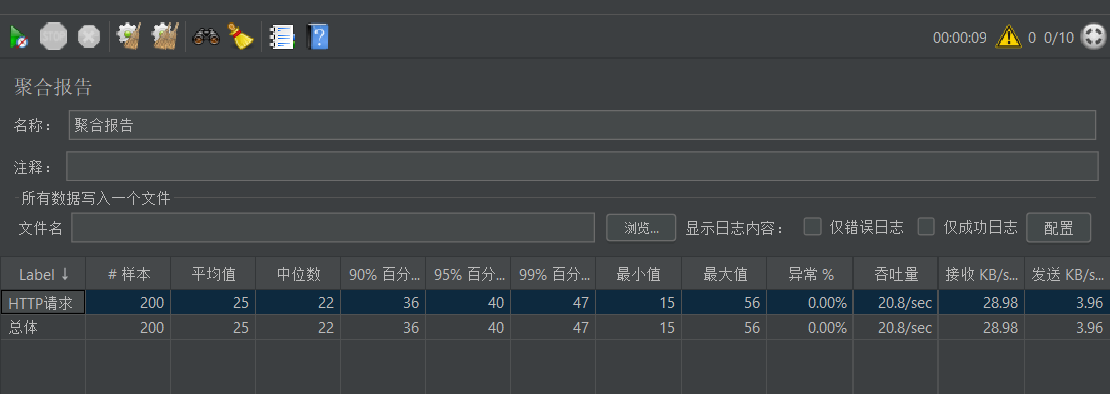
\includegraphics[width=0.96\textwidth]{figures/fig-6-1-forum-performance.png}
  \caption{论坛帖子查询接口聚合报告}
  \label{fig:forum-performance}
\end{figure}

拼车订单查询接口的聚合报告如\figref{fig:carpool-performance}所示。该接口平均响应时间为 198 ms，中位数为 188 ms，90\% 请求在 262 ms 内完成，最大响应时间为 495 ms，异常率同样为 0。与论坛接口相比，其耗时更高是符合预期的，因为接口除完成数据库查询外，还需要执行候选过滤、特征计算以及部分结果的模型重排。

\begin{figure}[!htbp]
  \centering
  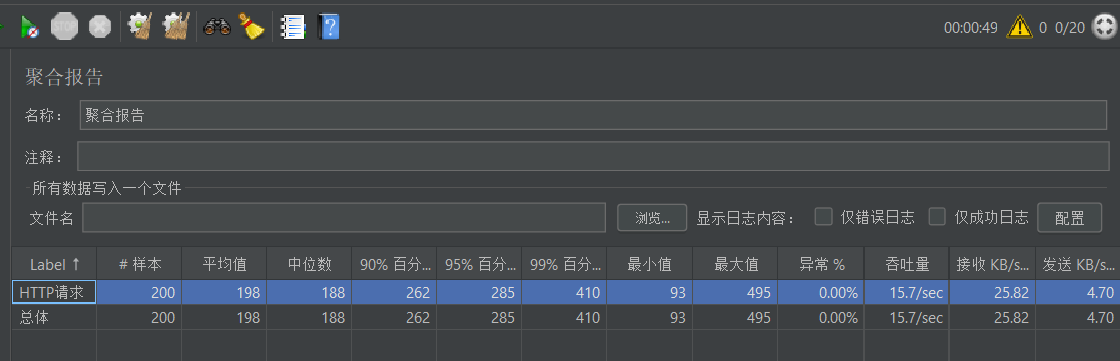
\includegraphics[width=0.96\textwidth]{figures/fig-6-2-carpool-performance.png}
  \caption{拼车订单查询接口聚合报告}
  \label{fig:carpool-performance}
\end{figure}

两组主要指标整理如表\ref{tab:performance-results}所示。

\begin{table}[!htbp]
  \caption{查询接口性能测试结果}
  \label{tab:performance-results}
  \centering
  \small
  \begin{tabular}{p{3.2cm}p{1.5cm}p{1.7cm}p{1.7cm}p{1.9cm}p{1.6cm}}
    \toprule
    测试接口 & 请求总数 & 平均响应时间/ms & 最大响应时间/ms & 90\%响应时间/ms & 异常率 \\
    \midrule
    论坛帖子查询接口 & 200 & 25 & 56 & 36 & 0.00\% \\
    拼车订单查询接口 & 200 & 198 & 495 & 262 & 0.00\% \\
    \bottomrule
  \end{tabular}
\end{table}

从结果看，论坛查询接口可以支持高频读取，拼车查询接口虽然耗时更高，但在给定并发条件下仍能稳定返回结果，且没有出现异常请求。对于当前规模的校园平台原型而言，这一表现能够满足日常使用需要。

\section{本章小结}

本章从单元测试、集成测试和系统测试三个层面对平台进行了验证。结果说明，系统主要业务链可以正常运行，接口交互基本稳定，拼车查询在包含规则筛选和模型排序的情况下仍保持可接受的响应水平。


